\documentclass[]{prezentare}
\graphicspath{{Imagini/}}

\title  {Operational monitoring of ATLAS TDAQ system}

\author [Cristian T\u al\u au]
        {\texorpdfstring
            {{\bf Autor:} Cristian T\u al\u au \\ 
            {\bf Supervisors:} Prof. Roger Hersch, Dr. Wainer Vandelli}
            {Cristian Talau}  
      }
\institute {\texorpdfstring{\href{http://epfl.ch}
                {\' Ecole Polytechnique F\' ed\' erale de Lausanne - EPFL}}
                {\' Ecole Polytechnique F\' ed\' erale de Lausanne - EPFL}}
                
\titlegraphic {
  
\includegraphics[scale=0.2]{../Images/epfl_logo.png} 
  $\,$
  
\includegraphics[scale=0.05]{../Images/cern_logo.png}}


\begin{document}

    \begin{frame}
        \titlepage
    \end{frame}

\begin{frame}
    \frametitle{Monitoring in the ATLAS TDAQ system}
    \begin{block}{Figures - global view}
    	\begin{itemize}
        	\item 15000 applications
        	\item running on 1500 nodes
            \item publish to 30 IS servers
      	\end{itemize}
  	\end{block}
    \begin{block}{Figures - single application}
    	\begin{itemize}
            \item publishes 5000 histograms
			\item with 500-1000 bins in average
            \item each histogram has a period between 5-120s
            \item 5-10 distinct periods in total
      	\end{itemize}
  	\end{block}
  	
\end{frame}

\begin{frame}[fragile]
     \frametitle{{\tt monsvc} Library}
     \begin{exampleblock}{Usage}
     	\begin{semiverbatim}
\alert<1>{ptr<TH1> phist = register("/DEBUG/event_size", &hist)}
\alert<2>{configure("/DEBUG/*", 30 * SEC, "DF")}
\alert<3>{start_publishing()}
...
\alert<4>{phist->update(event.size)}
...
stop_publishing()
        \end{semiverbatim}
	\end{exampleblock}
	\alt<2>{\begin{block}{Configuration}
	Provides a way to specify the publishing parameters associated with a given object.	
	\end{block}}{}
	\alt<3>{\begin{block}{Scheduling}
	Determines when to start publishing each histogram in each application.
	\end{block}}{}
	\alt<4>{\begin{block}{Synchronization}
	Ensures thread-safe access to the histogram for the application that updates it and the library thread which publishes.
	\end{block}}{}
\end{frame}

%-----------------------------------------------------------------------------------
\begin{frame}
	\frametitle{Configuration}
	\begin{block}
	
	\end{block}
\end{frame}
%-----------------------------------------------------------------------------------
\tikzstyle{every picture}+=[remember picture]

\begin{frame}[fragile]
	\frametitle{Synchronization}
	\begin{columns}
		\begin{column}{0.3\linewidth}
		
			\begin{block}{\tikz[baseline] \node (lt) {Library thread};}
				\begin{semiverbatim}
# lock:
\alert<2>{obj.lock()}

# unlock:
\alert<7>{with upd.lock: }
\alert<8>{  upd.exec()}
\alert<9>{  obj.unlock()}
				\end{semiverbatim}	
			\end{block}
		\end{column}

		\begin{column}{0.3\linewidth}
			\begin{tabular}{r l}
			{\tt obj} & 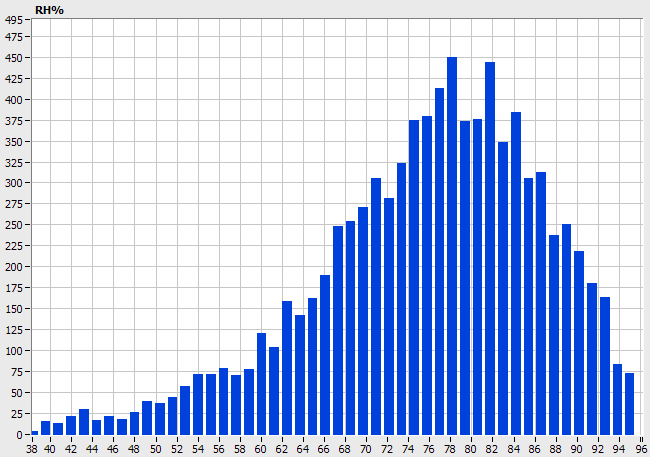
\includegraphics[scale=0.05]{../Images/histogram.png}
			\alt<2-9>{
			\begin{tikzpicture}[overlay]
				\node[yshift=5ex, xshift=-0.5ex] (objlock)
				  {
\includegraphics[scale=0.025]{../Images/lock.png}};
			\end{tikzpicture}
			}{} \\
			&\\
			{\tt upd} & \alt<6-8>{[(f,args)]}{[\, ]}
			\alt<3-14>{
			\begin{tikzpicture}[overlay]
				\node[yshift=1.75ex, xshift=-1ex] (updlock)
				  {
\includegraphics[scale=0.025]{../Images/lock.png}};
			\end{tikzpicture}
			}{} \\
			\end{tabular}	
		\end{column}
 		
		\begin{column}{0.4\linewidth}
			\begin{block}{\tikz[baseline] \node (mt) {Main thread};}
				\begin{semiverbatim}
# async(f, args):
\alert<3,10>{with upd.lock:}
\alert<4,11>{  if obj.try_lock():}
\alert<12>{    upd.exec()}
\alert<13>{    f(args)}
\alert<14>{    obj.unlock()}
\alert<5>{  else: }
\alert<6>{    upd.apnd(f, args)}
				\end{semiverbatim}
			\end{block}
		\end{column}
	\end{columns}

	\begin{tikzpicture}[overlay]
        \path<2-9>[->,thick] (objlock) edge [bend right] (lt);
        \path<3-6>[->,thick] (updlock) edge [bend left] (mt);
        \path<7-9>[->,thick] (updlock) edge [bend right] (lt);
        \path<11-14>[->,thick] (updlock) edge [bend left] (mt);
	\end{tikzpicture}

\end{frame}
%-----------------------------------------------------------------------------------
\begin{frame}
	\frametitle{Scheduling requirements}
	\begin{block}{Global}
		\begin{itemize}
			\item Minimize latency
			\item Minimize publishing skew
			\item Maximize throughput
		\end{itemize}
	\end{block}

	\begin{block}{Local}
		\begin{itemize}
			\item Minimize jitter
			\item Efficient reconfiguration
		\end{itemize}
	\end{block}
\end{frame}
%-----------------------------------------------------------------------------------
\begin{frame}
	\frametitle{Global scheduling}
	\begin{block}
	
	\end{block}
\end{frame}
%-----------------------------------------------------------------------------------
\begin{frame}
	\frametitle{Local scheduling}
	\begin{block}{Real-time system formulation}
	
	\end{block}
	\begin{block}{Offset-free system}
	
	\end{block}
\end{frame}
%-----------------------------------------------------------------------------------
\begin{frame}
	\frametitle{Local scheduling}
	\begin{block}{Subperiod algorithm}
		
	\end{block}
\end{frame}
%-----------------------------------------------------------------------------------
\begin{frame}
	\frametitle{Local scheduling}
	\begin{block}{Subperiod algorithm - results}
	
	\end{block}
\end{frame}
%-----------------------------------------------------------------------------------
    \begin{frame}
    \setbeamercolor{qa}{fg=block title.fg,bg=block title.bg} %structure.fg

    \begin{beamercolorbox}[rounded=true,shadow=true]{qa}
    \begin{center}
        {\Huge \textbf{Questions?}}
    \end{center}
    \end{beamercolorbox}
    \end{frame}

\end{document}
